\section{MODELAGEM DOS AMBIENTES DE SIMULAÇÃO}
\label{sec:modelagemAmbiente}

À modelagem do ambiente computacional utilizam-se \textit{shapefiles} como base de consulta às informações essenciais à representação em estruturas de dados dos ambientes georreferenciados escolhidos. É utilizado um recorte geográfico da cidade de Cascavel/PR.

Foram aplicados algoritmos para obtenção de vizinhanças diretamente sobre os pontos georreferenciados obtidos dos \textit{shapefiles}, resultando em uma descrição em grafos dos ambientes, em que as vizinhanças entre posições são apresentadas como arestas e os pontos georreferenciados os vértices do grafo. A utilização de uma estrutura de dados do tipo grafo possibilitou a flexibilização dos processos de obtenção das vizinhanças entre lotes e entre os pontos internos aos lotes. Os algoritmos desenvolvidos utilizam somente as informações referentes aos refinamentos dos lotes, a geometria dos polígonos que representam os lotes nos \textit{shapefiles} e as distâncias euclidianas entre os pontos georreferenciados. Adicionalmente, os processos de obtenção das vizinhanças entre lotes e ruas são automatizados por meio de consultas SQL ao banco de dados que armazena os \textit{shapefiles}, utilizando funções da extensão PostGIS. Na Seção \ref{sec:SIMULA} são apresentados detalhadamente as operações e consultas realizadas com o auxílio do banco de dados. 

São utilizados como base à especificação dos ambientes computacionais a cidade de Cascavel/PR que abrange $31$ bairros e $2.004$ quadras. Como na estrutura de dados presente na simulação considera-se os níveis de lote e quadra, os bairros foram mapeados para $32$ quadras e as quadras foram mapeadas para $3.672$ lotes. Foram inseridos uma quadra adicional e $1.668$ polígonos extras à representação das ruas entre quadras, com o objetivo de viabilizar os deslocamentos dos agentes entre as quadras do domínio. As Figuras \ref{fig:cascavel1} e \ref{fig:cascavel2} ilustram os \textit{shapefiles} da cidade de Cascavel/PR. 

\begin{figure}[H]
  \centering
  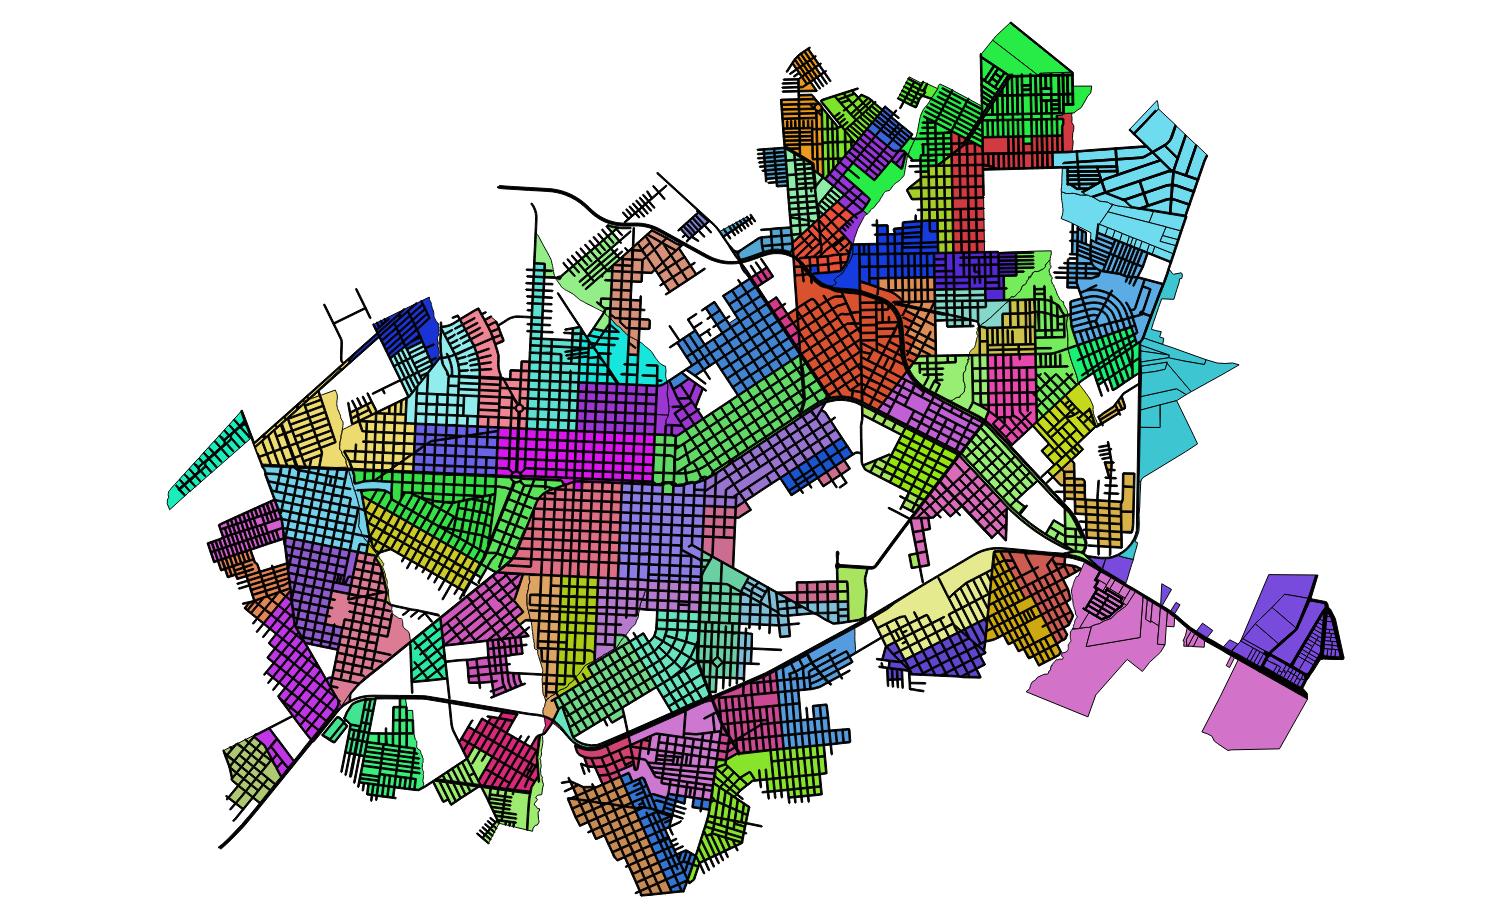
\includegraphics[width=0.8\textwidth]{Figuras/ModelagemAmbiente/Cascavel1.png}
  \caption{Representação gráfica do \textit{shapefile} da cidade de Cascavel/PR.}
  \label{fig:cascavel1}
\end{figure} 

\begin{figure}[H]
  \centering
  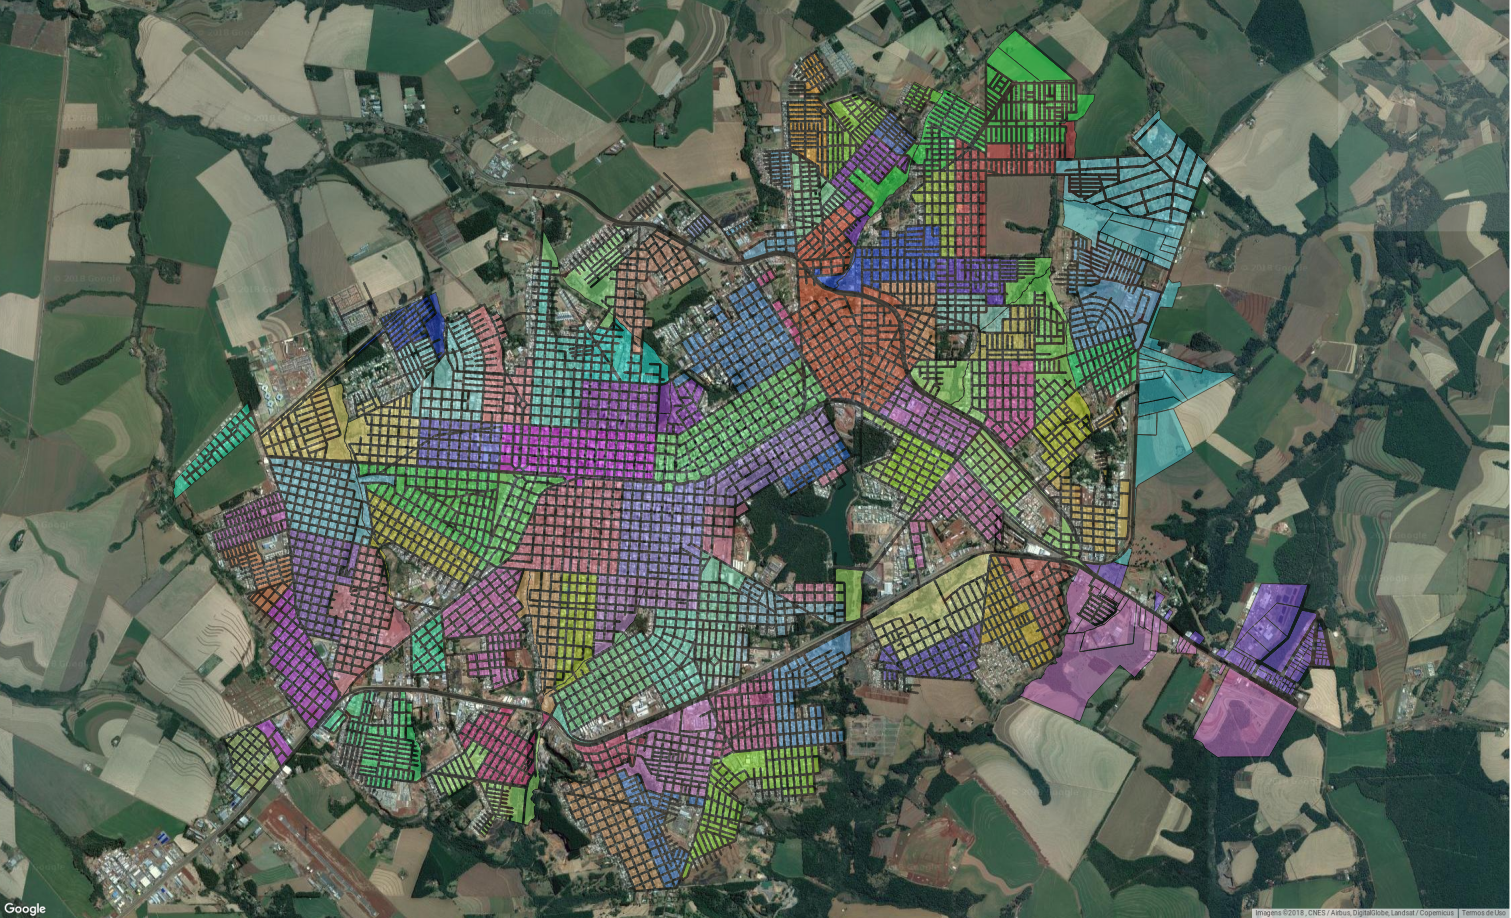
\includegraphics[width=0.8\textwidth]{Figuras/ModelagemAmbiente/Cascavel2.png}
  \caption{Representação gráfica do \textit{shapefile} da cidade de Cascavel/PR com fundo do Google Maps.}
  \label{fig:cascavel2}
\end{figure} 

A Seção \ref{sec:estruturasDadosEstrategiasImplementacao} apresenta detalhadamente as estruturas de dados e estratégicas empregadas na implementação do modelo apresentado. São apresentados ainda os operadores empregados à população de agentes, que são responsáveis pela evolução espaço-temporal da dinâmica da doença.

\newpage